% Page 038 — page imprimée 34
% Contenu seul : le préambule et la pagination sont gérés par meyrueis.tex


L’année suivante, dès mon arrivée à Meyrueis, je montai à la Bergerie : la porte était toujours
sans serrure, rien ne s’opposait à une nouvelle exploration. Mon cousin n’était pas là mais
c’était sans importance. J’étais bien décidé à faire moi-même mes découvertes sans en parler à
personne, car j’avais une idée : je voulais explorer la cheminée dont nous avions vu l’entrée
au dessus de la vasque. Trois jours plus tard l’occasion se présenta : le temps était beau, ma
tante avait des visites à faire et je lui annonçais que j’allais en promenade. J’avais 3 bougies,
une lampe électrique et 2 boîtes d’allumettes. Quelques minutes après, j’étais sur les lieux
sans soupçonner que j’étais au seuil d’une expérience décisive…
Rien n’avait changé depuis l’année précédente : la terre de nos déblais se trouvait toujours à
l’entrée de notre tunnel. Lorsque je m’y glissais je retrouvais le sentiment délicieux qui me
saisissait autrefois lorsque je jouais à me perdre sous les couvertures du lit de mes parents. À
la sortie, je retrouvais le fil rouge que nous avions attaché à une stalagmite. Je descendis sans
anicroche, retrouvais la vasque et sa cheminée qui n’était pas d’un accès difficile. Je
l’escaladais sans hésiter, et à moins de 2 m. je rencontrais une galerie horizontale, assez large
qui s’ouvrait à droite et à gauche. Les parois étaient lisses le sol uni : elle avait servi de canal
il y a quelques dizaines de milliers d’années et la cheminée était le résultat d’une dislocation
sans doute provoquée par un tremblement de terre ; ses roches brutes n’avaient pas été usées
par les eaux du canal probablement tari par la même occasion. Suivant alors la galerie je
découvris d’autres fissures dans le sol. Pour épargner la lampe électrique j’avais allumé une
bougie. J’avançais pas à pas, prudemment… Soudain je me trouvais au seuil d’une
merveille !!! C’était une salle relativement petite, intime et ronde, comme un petit salon,
entièrement tapissée de cristaux brillants et translucides. J’allumai des deux autres bougies :
leur lumière était réfléchie mille, dix mille fois en faisceaux irisés d’étincelantes couleurs. Ma
présence dans cet écrin me semblait presque sacrilège, j’étais fasciné immobile tout entier
dans la joie de l’admiration.

Cinquante six ans plus tard en 1977, lors d’une courte visite à Meyrueis, j’essayai de retrouver
la bergerie. Le chemin existait toujours quoique embroussaillé mais le petit champ était
clôturé et avait une porte neuve fermée à clé. Et la tranchée qui menait à l’entrée de la grotte
avait été soigneusement remplie sur toute sa longueur par des branchages aux épines acérées.

Ma grotte était condamnée, plus dangereuse peut-être que je ne l’avais cru. Dommage...

J’aurais aimé pouvoir retrouver, ne fut-ce que pour un moment, l’obscurité totale et le
silence, un silence ponctué depuis toujours par la chute d’une goutte d’eau dans une vasque,
la même... jamais la même ! ».


\begin{center}
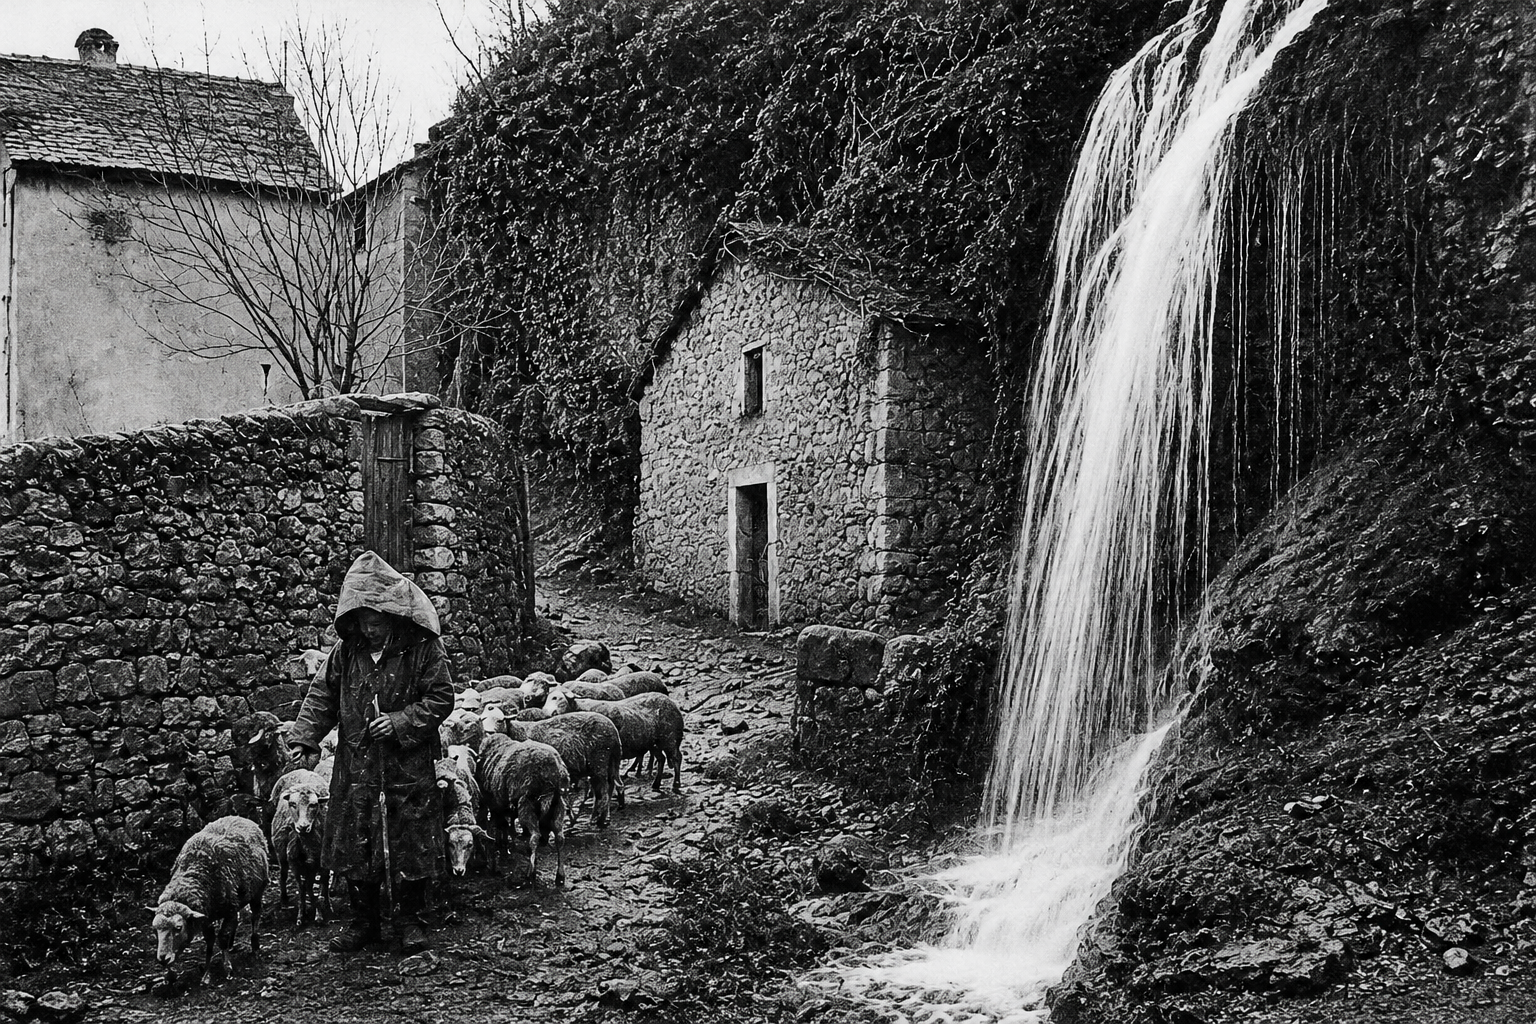
\includegraphics[width=0.78\textwidth]{imgs/040.png}
\end{center}
